
\chapter{General-Purpose Computing on Graphics Processing Units}
General-Purpose computing on graphics processing unit (GPGPU) is the use of graphics processing unit (GPU) and central processing unit (CPU) together for acceleration data-intensive or compute-intensive tasks. Main advantage of GPUs is that in comparison with ordinary CPU, they have ten times, a hundred times but sometimes thousand times more cores, so if the task is parallelizable, it could be accelerated up to thousand times on GPU in comparison to serial CPU version. At the beginning, GPUs support only computation of vectors or matrices, usually two, three or four dimensional for graphical purposes, so general purpose computation had to be reformulated to this graphical principles supported by major graphics APIs like DirectX or OpenGL. Later, Nvidia CUDA and OpenCL frameworks solve this problem and allows to programmer to ignore graphics environment. Main difference between this two frameworks is that CUDA is only for Nvidia graphics cards so it could use concrete hardware specific properties. OpenCL is a universal vendor independent framework for parallel computations and can be run on wide range of devices like GPUs and CPUs, but , but it is not so good for high performance computing as CUDA because of wide range of covered devices so it could not use architecture and hardware specific properties.
\subsection{GPU and CPU comparison} \label{ssec:gpucpucomparison}
Main difference between CPU and GPU is in their specialization. Instead of general purpose of CPUs, GPUs are specialized on graphics, which is easily parallelizable, so GPU architecture is targeted for parallel work. After GPGPU was introduced, problem with GPU specialization was solved and GPUs began to compete with processors. Main differences between CPUs and GPUs are:
\begin{description}
\item[Number of cores] CPU has only few physical cores~\autoref{fig:cpuarchitecture}, sometimes virtually doubled. Common home CPUs have a maximum around 8 logical cores, server CPUs could have more, but maximally slightly less than a hundred cores. Compared two that, modern GPUs have around five hundred cores~\autoref{fig:gpuarchitecture}, the best models have around five thousand cores, so they have great potential for parallel tasks.
\item[Core architecture] GPU cores are specialized for numeric computations, not for general tasks as CPU cores, but because of their specialization, they compute numeric tasks really fast. \item[Threads] Approach to threads is different. CPU can process threads from different tasks at one time, which is called Simultaneous Multithreading (SMT), GPU uses Simple Instruction Multiple Thread (SIMT) pattern, which means that multiple threads run on same code and based on their identification, they could work on different branches or access different data.
\item[Memory] CPUs use big cache memory for hide latency of memory access so when thread is switched to different core, there is problem witch locally cached data, which are useless on original core and must be re-cached on new core. GPU has only small caches, because most of memory is on device, so context switch can be performed really fast.

\begin{figure}[h]
\centering
\begin{subfigure}{.5\textwidth}
  \centering
  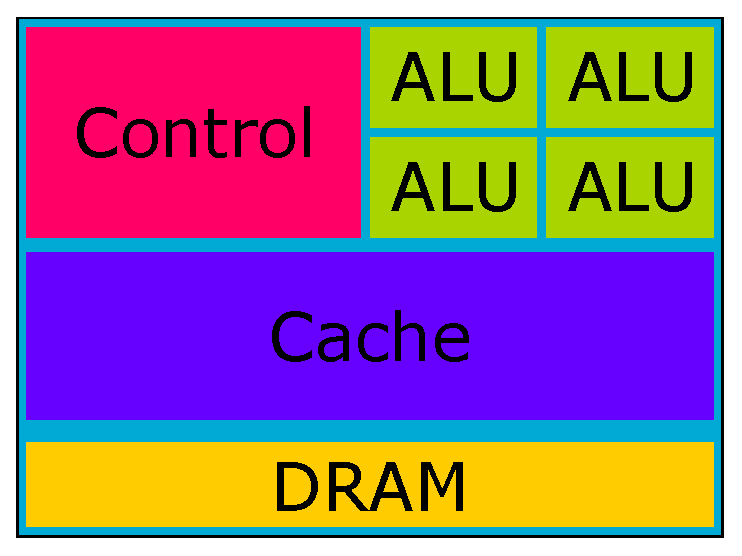
\includegraphics[width=.8\linewidth]{img/CPUarchitecture.eps}
  \caption{CPU architecture}
  \label{fig:cpuarchitecture}
\end{subfigure}
\begin{subfigure}{.5\textwidth}
  \centering
  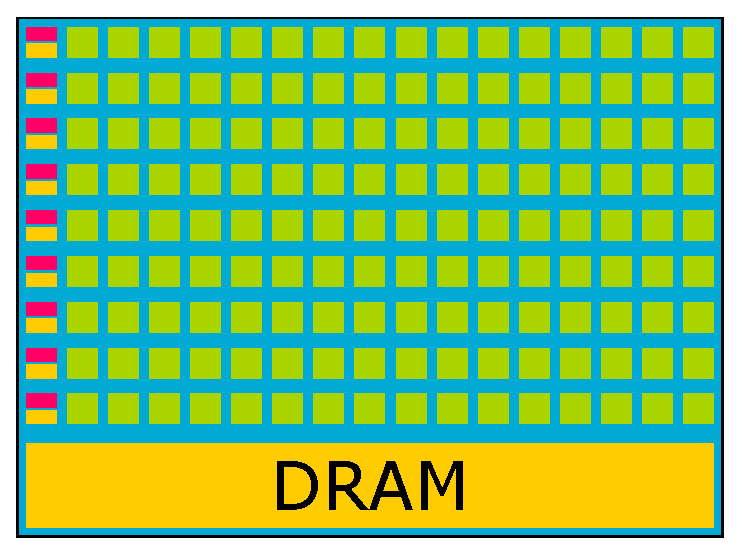
\includegraphics[width=.8\linewidth]{img/GPUarchitecture.eps}
  \caption{GPU architecture (Fermi)}
  \label{fig:gpuarchitecture}
\end{subfigure}
\caption{CPU and GPU architecture comparison}
\end{figure}

\end{description}
%\begin{table}
%\begin{tabular}{|l|l|l|}
%\cline{1-2}
%NIC & CPU & GPU \\ \cline{1-2}
%# cores & Few cores per chip & Many cores per chip \\ \cline{1-2}
%Specialization & General purpose cores & Cores psecialized for numeric computations \\ \cline{1-2}
%Threads approach & Processing different threads & SIMT thread processing \\ \cline{1-2}
%Memory access & Huge caches to reduce memory latency & Huge amount of threads and fast context switch \\ \cline{1-2}
%\end{tabular}
%\end{table}
\subsection{Compute Unified Device Architecture (CUDA)}
CUDA is parallel computing platform developed by Nvidia. This includes hardware and software architecture integrated on Nvidia graphics cards. There exist more solutions than this one from Nvidia, but CUDA is one of the best for high performance computing. The main advantage over OpenCL and other solutions is a direct link to the hardware, which is not the case of OpenCL, because it supports a large range of hardware divergent devices so it can't use concrete hardware advantages. \\
Nvidia use Simple Instruction Multiple Thread (SIMT) model, which is more flexible than Simple Instruction Multiple Data (SIMD), but generally, it has less performance. Both models approaching parallelism by by broadcasting same instruction to multiple execution units, so only one instruction fetch/decode unit is needed by many execution units. Difference is that SIMT also have multiple register sets and addresses. Main difference is that SIMD processes short vectors in parallel and always all threads do the same work. For example, when we need sum two vectors, SIMD must iterate through vectors and in one step, it can only process as many elements as a computing units count is. On CUDA with SIMT model, we launch as many threads as size of vector and each thread can store values in own register. Not all threads run actually in parallel, but many of them do.\\
CUDA architecture contains larger processors called \textbf{Symmetric Multiprocessor (SM)}. The oldest is \textbf{SMP} - Fermi~\autoref{fig:smparchitecture}, \textbf{SMX} - Kepler~\autoref{fig:smxarchitecture} and the newest \textbf{SMM} - Maxwell~\autoref{fig:smmarchitecture}. Each SMP contains processor cores with registers (from 32 on Fermi architecture, 128 on Maxwell architecture and 192 on Kepler architecture), load/store units (LD/ST), Special Function Units (SFUs), shared instruction cache, shared memory and data caches. LD/ST and SFUs are shared by groups of cores, size of group depends on architecture.\\
Versions of CUDA are referred as \textbf{Compute Capability} (CC). This CC describe the device characteristics and a set of instructions that are supported. CC is tightly coupled with architecture (CC 1.x was supported by Tesla architecture, CC 2.x by Fermi, 3.x by Kepler, 5.x by Maxwell).

\subsubsection{Execution model}

\begin{figure}[h]
  \centering
  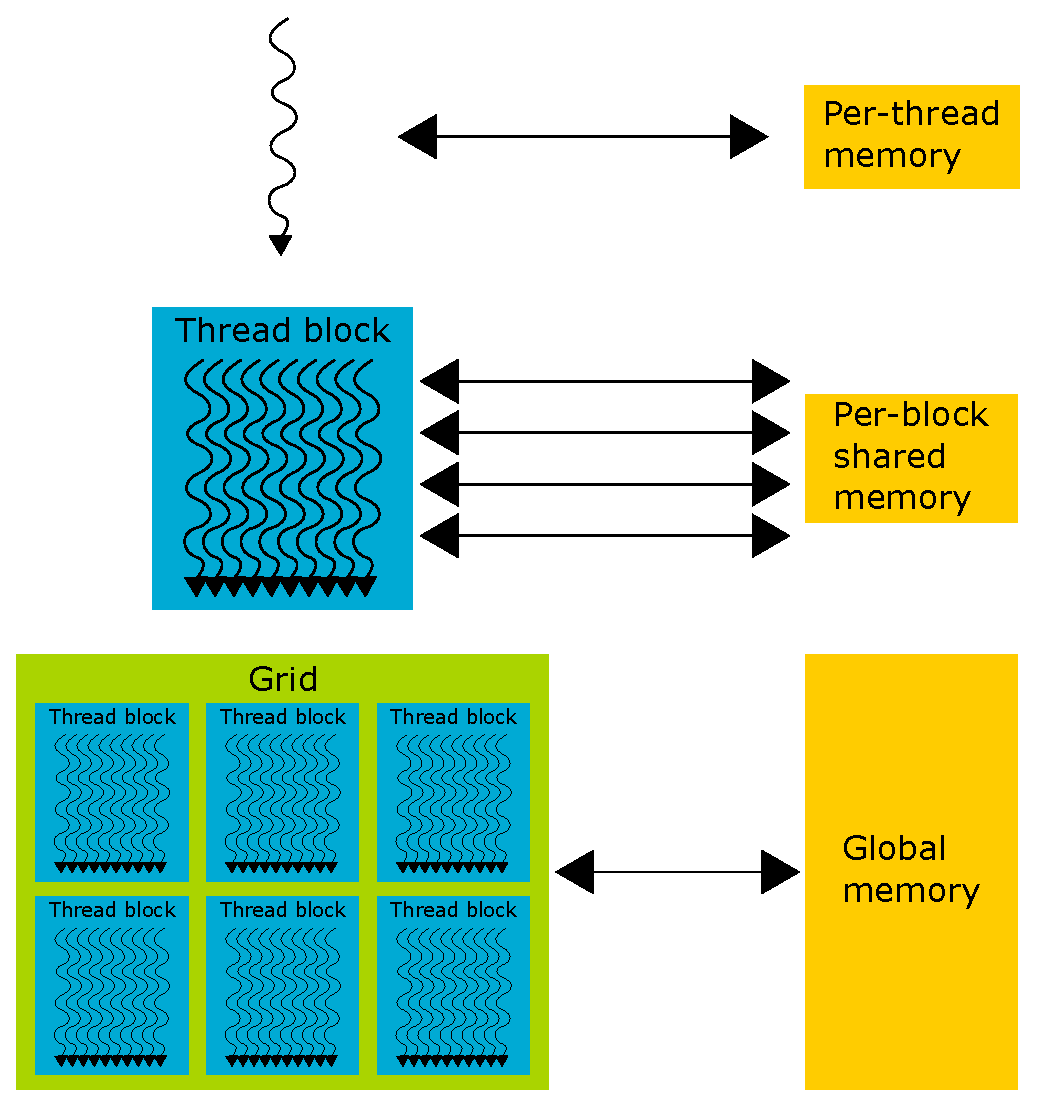
\includegraphics[width=0.8\linewidth]{img/CUDAExecutionModel.eps}
  \caption{CUDA Execution model}
  \label{fig:cudaexecmodel}
\end{figure}

Parallel programming on CUDA architecture contains two layers of parallelization~\autoref{fig:cudaexecmodel}. The first layer of parallelization is called \textbf{Grid} and it is handled by single GPU chip. Grid consists of blocks which are mapped to Symmetric Multiprocessors, each SM handle one or more \textbf{blocks} but block is never handled by more than one SM. The second layer (Block) consist of \textbf{threads} which runs on cores. The block size could be even bigger than number of cores on SM, than only part of block is run simultaneously. This part is called \textbf{Warp}.\\ Maximum number of currently running blocks and threads in each block depends on architecture, because each architecture has different number of SMs and SM has different number of compute cores. Threads in one block could be executed concurrently or serially and no particular order, but it can be coordinated by synchronizing threads.\\

\begin{figure}[p]
\centering
\begin{subfigure}{0.49\textwidth}
  \centering
  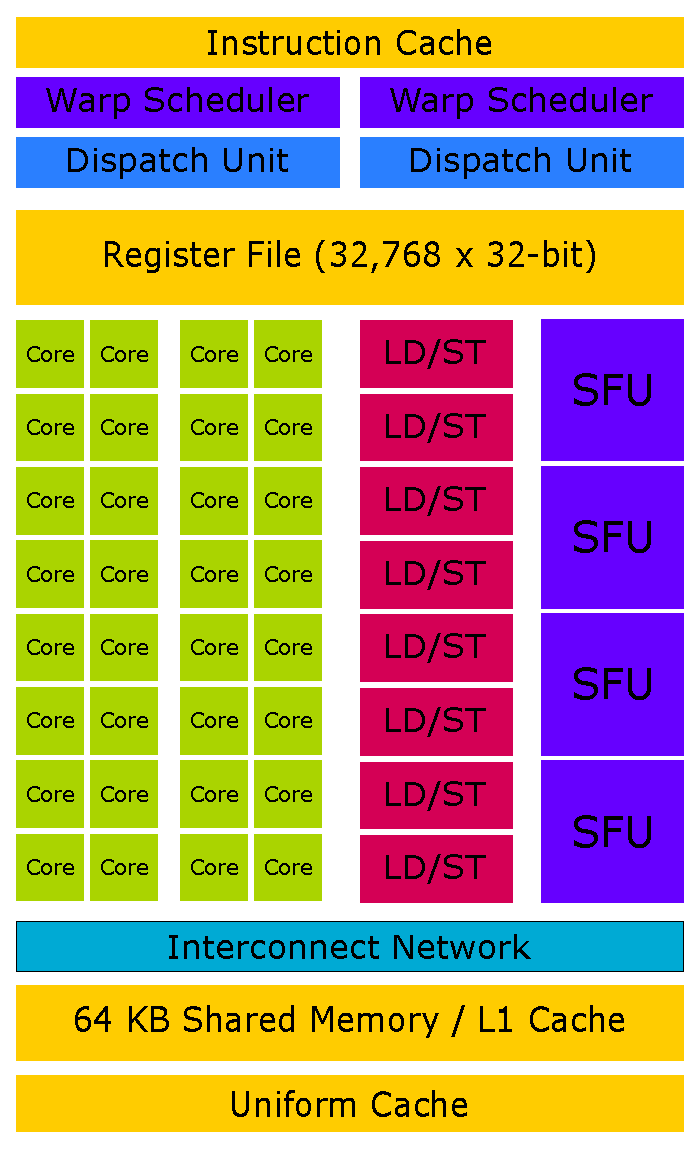
\includegraphics[width=0.8\linewidth]{img/SMPArchitecture.eps}
  \caption{SMP architecture}
  \label{fig:smparchitecture}
\end{subfigure}
\begin{subfigure}{0.49\textwidth}
  \centering
  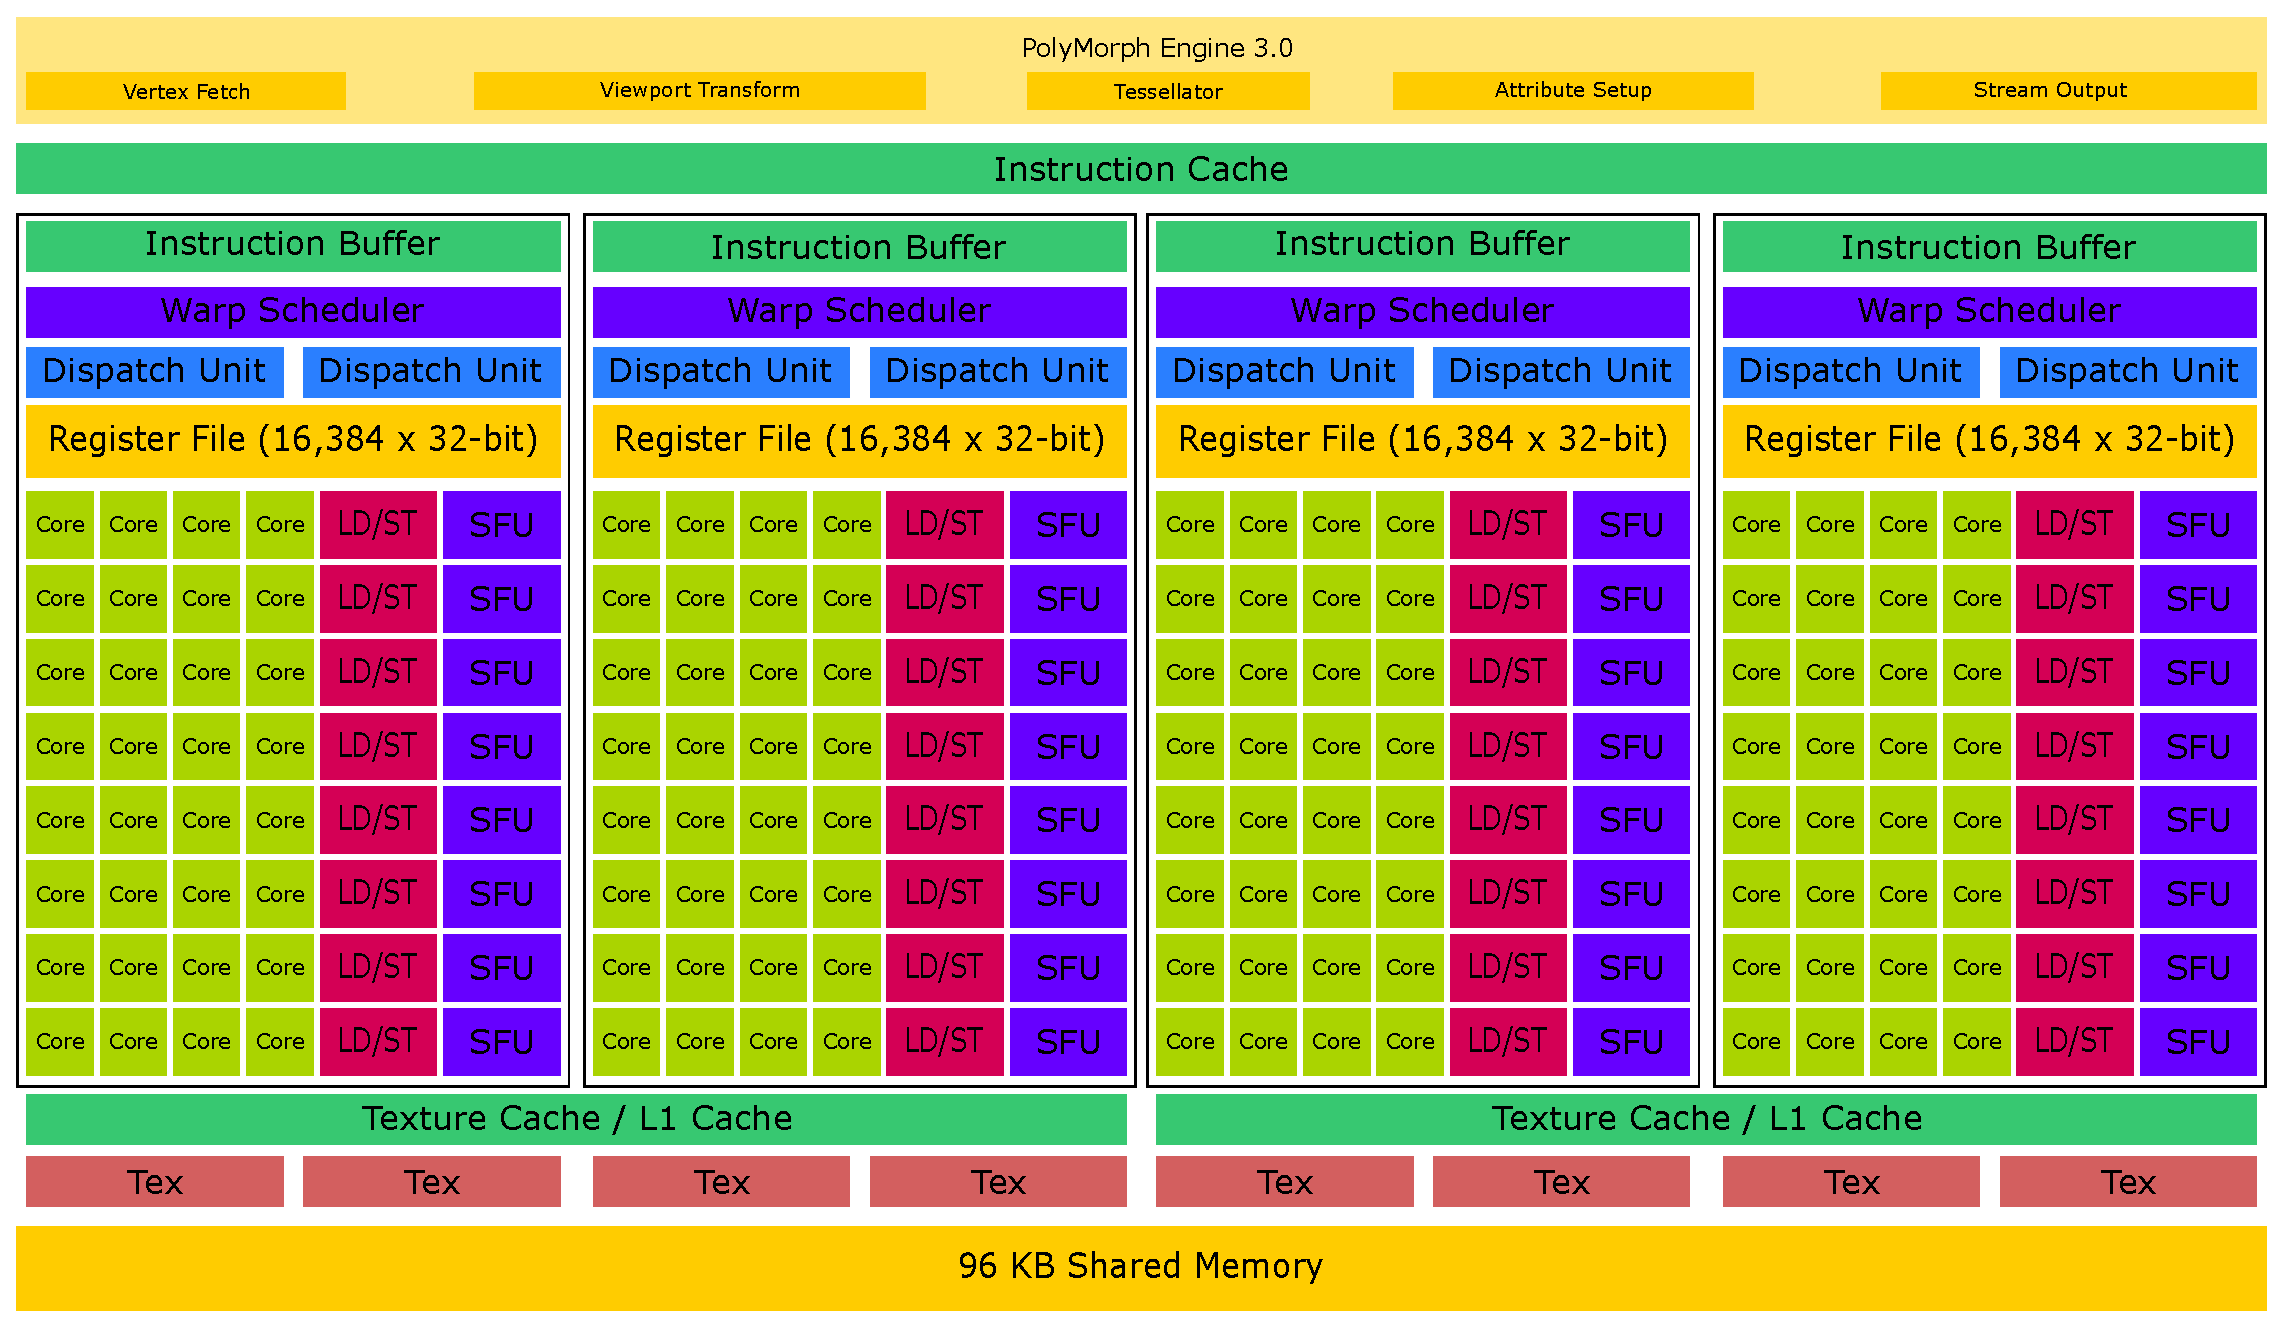
\includegraphics[width=1\linewidth]{img/SMMArchitecture.eps}
  \caption{SMM architecture (Fermi)}
  \label{fig:smmarchitecture}
\end{subfigure}
\vspace*{0.1cm} 
\begin{subfigure}{0.6\textwidth}
  \centering
  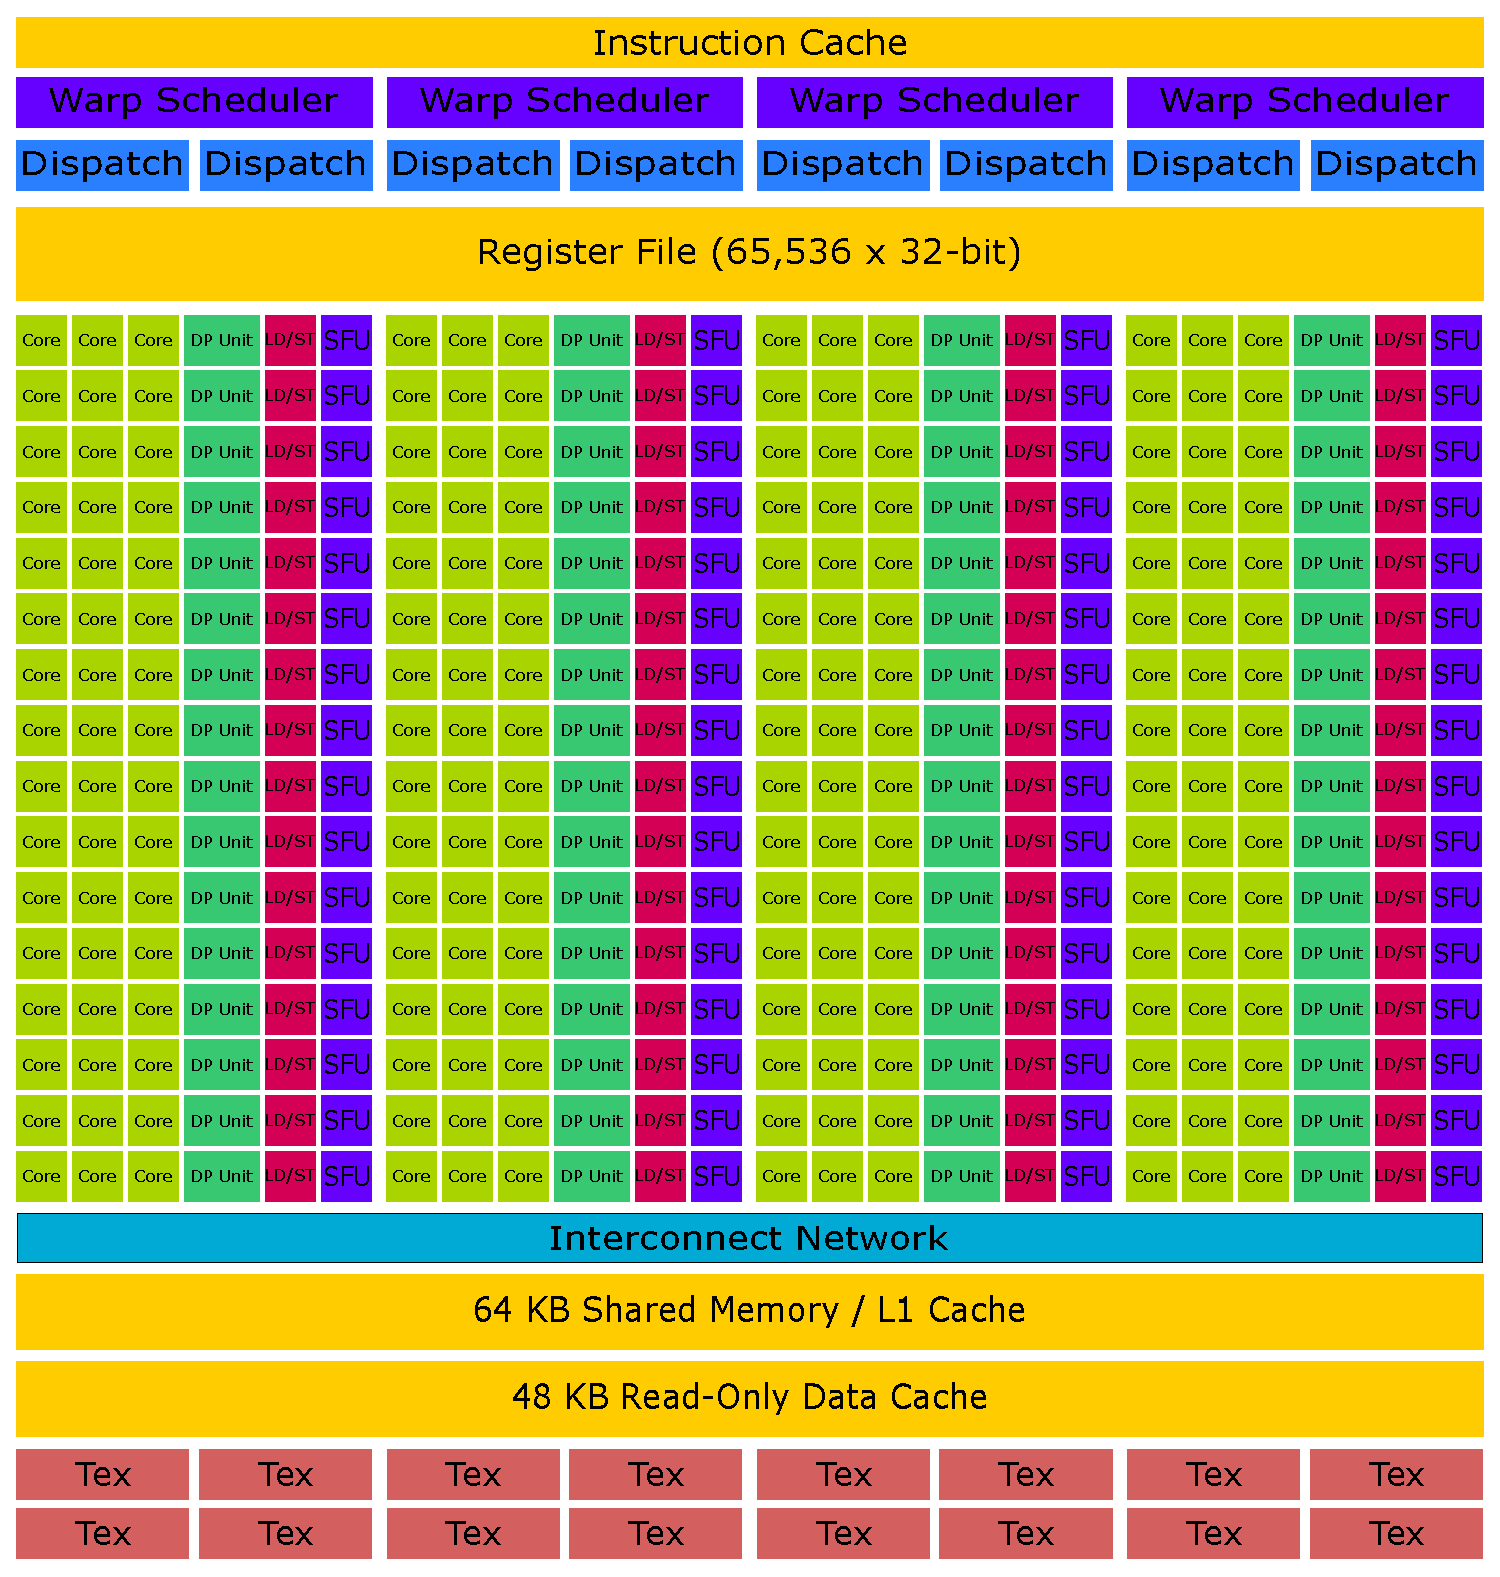
\includegraphics[width=0.9\linewidth]{img/SMXArchitecture.eps}
  \caption{SMX architecture (Fermi)}
  \label{fig:smxarchitecture}
\end{subfigure}
\caption{CPU and GPU architecture comparison}
\end{figure}

\subsubsection{Memory model}

Memory model on CUDA architecture~\autoref{fig:cudamemaccess} contains more types of memory which differs mainly in size, bandwidth and latency.
\begin{description}
\item[Global memory] is off the chip, but on the device. It is the largest memory (GBs) and it has high bandwidth (~100 GBps) but high latency (400-600 clock cycles). It is operated in transactions of 32B - 128B and data are cached in L2 cache. Global memory is accessible from all threads.
\item[Shared memory] is memory is shared by all threads running on same SM. It has lower latency (32 bits / 2 cycles on CC 1.x and 2.x and 64 bits / 1 cycle on 3.x) than Global memory, but it is also smaller (depend on Compute Capability, from 16 kB on 1.x CC to 48kB on 2.x CC and 3.x CC). This memory is divided into banks, each bank could be accessed independently. If there are conflicts, access to bank is serialized (except reading same address which is called broadcast). On CC 1.x and CC 2.x, bank size is 32 bits, on CC 3.0 we can select between 32 bits and 64 bit banks.
\item[L1 Cache] has on most devices similar parameters as Share memory, because it has same resource. We can configure which memory should be preferred and bigger. On CC 3.0, L1 cache was merged with texture cache and is independent on shared memory (resources are not shared).
\item[Registers] Each multiprocessor has own register pool. Depend on CC, it has 8-64k of 32-bit registers. registers are the smallest memory, but also has the smallest latency (they are as fast as cores). For programmer, registers are not directly controllable. Only slow down is read-after write dependency which takes 24 clock cycles, but it could be hidden by enough of active warps.
\item[Local memory] is memory used only by single thread. Bigger data structures and arrays are stored here because they don't fit into registers. Because of smaller register size, some of registers are deferred in local memory.
\item[Constant memory] is a special memory for read-only data. Its size is 64kB and from CC 2.x, compiler stores here constant, thread-independent variables.
\item[Texture memory] is special memory used for graphics. Its main benefit is 2D spatial locality used mainly for textures.
\end{description}

\begin{figure}[h]
  \centering
  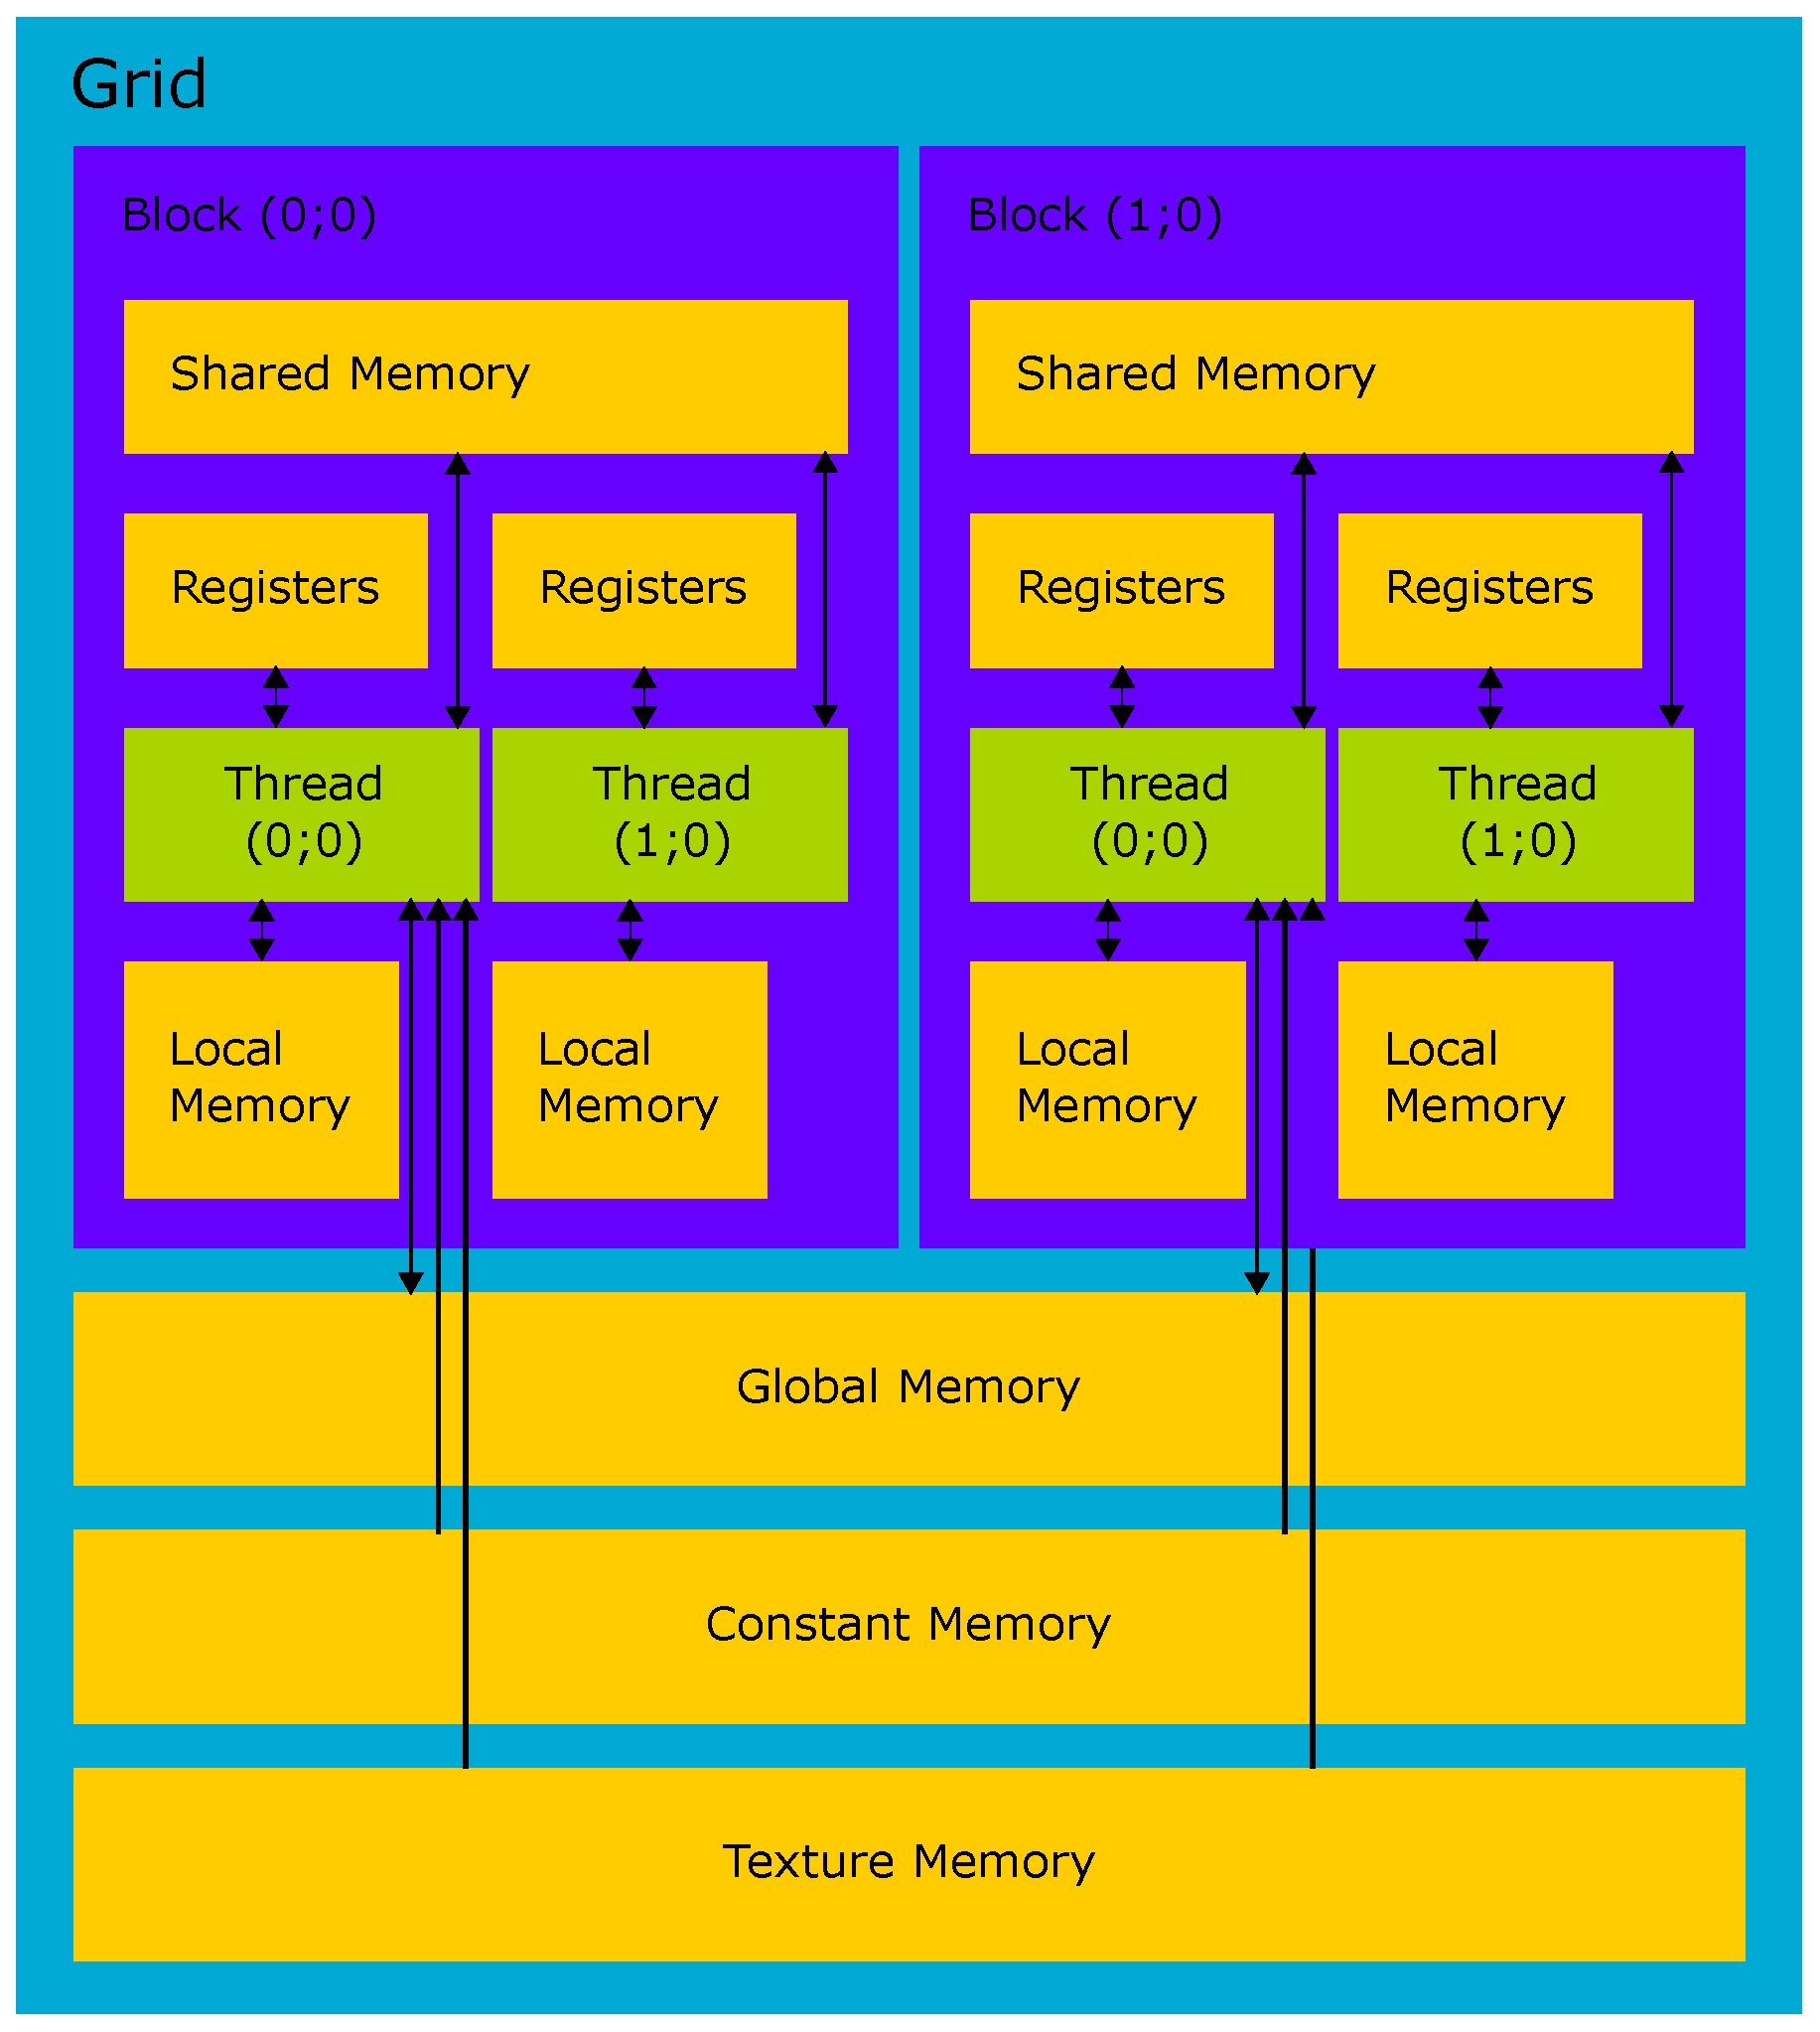
\includegraphics[width=0.6\linewidth]{img/CUDAmemAccess.eps}
  \caption{CUDA Memory access}
  \label{fig:cudamemaccess}
\end{figure}

Data transfer between host and device are much slower than on device memory transfers (16/32 GBps depend on PCI Express version, but could be slowed by host memory), which could make CUDA inefficient for small data and compute inexpensive tasks. Transfer call has great overhead so bulk transfers are preferred over individually transfers. Data are copied from host code to device global memory but host memory could be mapped to the host memory space and than data could be accessed directly from device code (but with same, bad latency). Data transfer could be hidden by overlapping data transfer with computing, because CUDA device is capable of computing and simultaneously perform two asynchronous data transfers.

% is little bit different, because programmer can split execution of instructions into different branches by conditions based on thread identification. In both models